\begin{exercises} 

\item \label{Ez:9.2.1}   Let $\vv = \langle 1, -2 \rangle$, $\vu = \langle 0, 4 \rangle$, and $\vw = \langle -5, 7 \rangle$.
%\begin{figure}[h]
%\begin{center}
 %\includegraphics{figures/1_1_Ez1.eps}
 %\caption{A bungee jumper's height function.} \label{F:1.1.Ez1}
%\end{center}
%\end{figure}

    \ba
    	\item Determine the components of the vector $\vu - \vv$.
        \item Determine the components of the vector $2\vv - 3\vu$.
        \item Determine the components of the vector $\vv + 2\vu - 7 \vw$.
        \item Determine scalars $a$ and $b$ such that $a \vv + b\vu = \vw.$
    \ea

\begin{exerciseSolution}
    \ba
    	\item In this example we have $\vu - \vv = \langle 0-1, 4-(-2) \rangle = \langle -1, 6 \rangle$.
        \item In this example we have $2\vv - 3\vu = \langle 2(1)-3(0), 2(-2)-3(4) \rangle = \langle 2, -16 \rangle$.
        \item In this example we have $\vv + 2\vu - 7 \vw = \langle 1+2(0)-7(-5), -2+2(4)-7(7) \rangle = \langle 36, -43 \rangle$.
        \item Since $a \vv + b\vu = \langle a, -2a+4b \rangle$, in order for $a \vv + b\vu$ to equal $\vw$ we must have $a=-5$ and $-2(-5)+4b = 7$. So $a=-5$ and $b = -\frac{3}{4}$.  
    \ea
\end{exerciseSolution}


\item \label{Ez:9.2.2}  Let $\vu = \langle 2, 1 \rangle $ and $\vv = \langle 1, 2 \rangle$.


    \ba
    \item Determine the components and draw geometric representations of the vectors $2\vu$, $\frac{1}{2}\vu$, $(-1)\vu$, and $(-3)\vu$ on the same set of axes.

    \item Determine the components and draw geometric representations of the vectors $\vu + \vv$, $\vu + 2\vv$, and $\vu + 3\vv$.
    
    \item Determine the components and draw geometric representations of the vectors $\vu - \vv$, $\vu - 2\vv$, and $\vu - 3\vv$.
    
    \item Recall that $\vu - \vv = \vu + (-1)\vv$.  Use the ``tip to tail'' perspective for vector addition to explain why the difference $\vu - \vv$ can be viewed as a vector that points from the tip of $\vv$ to the tip of $\vu$.
    
   
    \ea

\begin{exerciseSolution}
    \ba
    \item Here we have 
\begin{align*}
2\vu &= \langle 4,2 \rangle \\
\frac{1}{2}\vu &= \left\langle 1, \frac{1}{2} \right\rangle \\
(-1)\vu	&= \langle -2, -1 \rangle \\
(-3)\vu &= \langle -6, -3 \rangle.
\end{align*}
Pictures of these vectors, all of which lie on the same line, are shown in the figure below. 
\begin{center}
\resizebox{!}{2.0in}{\includegraphics{9_2_Ex_2_a}}
%\includegraphics{figures/9_2_Ex_2_a}
\end{center}


    \item Here we have 
\begin{align*}
\vu + \vv &= \langle 3,3 \rangle \\
\vu + 2\vv &= \langle 4, 5 \rangle \\
\vu + 3\vv	&= \langle 5, 7 \rangle.
\end{align*}
Pictures of these vectors, whose terminal points all lie on the same line, are shown in the figure below. 
\begin{center}
\resizebox{!}{2.0in}{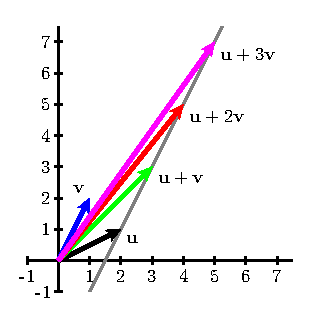
\includegraphics{9_2_Ex_2_b}}
\end{center}
    
    \item Here we have 
\begin{align*}
\vu - \vv &= \langle 1,-1 \rangle \\
\vu - 2\vv &= \langle 0, -3 \rangle \\
\vu - 3\vv	&= \langle -1, -5 \rangle.
\end{align*}
Pictures of these vectors, whose terminal points all lie on the same line, are shown in the figure below. 
\begin{center}
\resizebox{!}{2.0in}{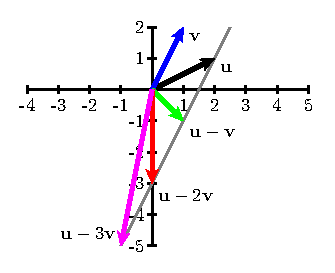
\includegraphics{9_2_Ex_2_c}}
\end{center}

   
    \item The figure below illustrates that $\vu - \vv = \vu + (-1)\vv$ is the same as the vector from the tip of $\vv$ to the tip of $\vu$.
\begin{center}
\resizebox{!}{2.0in}{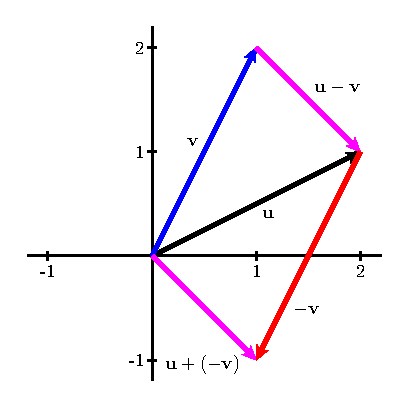
\includegraphics{9_2_Ex_2_d}}
\end{center}   
   
    \ea
\end{exerciseSolution}


\item \label{Ez:9.2.3}  Recall that given any vector $\vv$, we can calculate its length, $|\vv|$.  Also, we say that two vectors that are scalar multiples of one another are \emph{parallel}. 


    \ba
    \item Let $\vv = \langle 3,4 \rangle$ in $\R^2$.  Compute $|\vv|$, and determine the components of the vector $\vu = \frac{1}{|\vv|} \vv$.  What is the magnitude of the vector $\vu$?  How does its direction compare to $\vv$?
    
    \item Let $\vw = 3\vi - 3\vj$ in $\R^2$.  Determine a unit vector $\vu$ in the same direction as $\vw$.
    
    \item Let $\vv = \langle 2, 3, 5 \rangle$ in $\R^3$.  Compute $|\vv|$, and determine the components of the vector $\vu = \frac{1}{|\vv|} \vv$.  What is the magnitude of the vector $\vu$?  How does its direction compare to $\vv$?

    \item Let $\vv$ be an arbitrary nonzero vector in $\R^3$. Write a general formula for a unit vector that is parallel to $\vv$.

    \ea

\begin{exerciseSolution}
    \ba
     \item We know that $|\vv| = \sqrt{3^2+4^2} = 5$. So $\vu = \frac{1}{|\vv|} \vv = \left\langle \frac{3}{5}, \frac{4}{5} \right\rangle$. The magnitude of $\vu$ is $|\vu| = \sqrt{\left(\frac{3}{5}\right)^2 + \left(\frac{4}{5}\right)^2} = 1$. Since $\vu$ is a positive scalar multiple of $\vv$, the vector $\vu$ is a unit vector in the direction of $\vv$. 
    
    \item As in part (a), to find a unit vector in the direction of $\vw$, we divide $\vw$ by its magnitude. So a unit vector $\vu$ in the same direction as $\vw$ is $\vu = \frac{1}{|\vw|} \vw = \frac{1}{\sqrt{18}} \vw = \left\langle \frac{3}{\sqrt{18}}, -\frac{3}{\sqrt{18}} \right\rangle$.
    
    \item We know that $|\vv| = \sqrt{2^2+3^2+5^2} = \sqrt{38}$. So $\vu = \frac{1}{|\vv|} \vv = \left\langle \frac{2}{\sqrt{38}}, \frac{3}{\sqrt{38}}, \frac{5}{\sqrt{38}} \right\rangle$. The magnitude of $\vu$ is $|\vu| = \sqrt{\left(\frac{2}{\sqrt{38}}\right)^2  + \left(\frac{3}{\sqrt{38}}\right)^2 + \left(\frac{5}{\sqrt{38}}\right)^2} = 1$. Since $\vu$ is a positive scalar multiple of $\vv$, the vector $\vu$ is a unit vector in the direction of $\vv$. 

    \item If $\vv$ is an arbitrary nonzero vector in $\R^3$, then the vector $\frac{1}{|\vv|} \vv$ is a unit vector that is parallel to $\vv$.

    \ea
\end{exerciseSolution}

\end{exercises}

\afterexercises
